\section{Empirical Application}
In this section we are going to apply our CV model averaging method and other related methods to forecasting the quarterly GDP growth rate for the U.S. and Taiwan. These two series are shown in figure~\ref{fig1}. The U.S. data is obtained from the Bureau of Economic Analysis\footnote{\url{http://www.bea.gov/}}. The data for Taiwan is from National Statistics\footnote{\url{http://eng.stat.gov.tw/}}. The U.S. series is shown in the blue colored solid line while the Taiwan series is denoted in red colored dash line. Note that the data for Taiwan is shorter than that of the the U.S. This is because Taiwan officially starts its modernization with American aid in the early 1950s.

For the U.S. series, we can see that the growth rate becomes less volatile toward the end of the sample. This is the so called Great Moderation phenomenon, see Stock \cite{Stock_DEECON2004} and Stock and Watson \cite{Stock_Watson_JEL2003}. Stock and Watson argue that the forecasting relationship for the GDP growth is time-varying and combination forecasts reliably improve upon the AR benchmark. They claim ``\emph{From the perspective of forecasting methods, this evidence of sporadic predictive content poses the challenge of developing methods that provide reliable forecasts in the face of time-varying relations...the finding that averaging individually unreliable forecasts produces a reliable combination forecast is not readily explained by the standard theory of forecast combination, which relies on information pooling in a stationary environment...fully articulated statistical or economic models consistent with this observation could help to produce combination forecasts with even lower MSFEs.}'' In the next section, we demonstrate that our theory based CV model averaging method performs better than Mallows' weight, Bayesian weight, and most importantly, the equal weight method in terms of smaller root MSFE.

For the Taiwan series, we can see that it has two interesting features. First, it looks like that the average growth rate has dropped toward the end of the sample. This could be explained by the economic growth theory in Macroeconomics that during the early period of modernization or industrialization, a country tends to have high GDP growth rate. But as time goes, the growth rate approaches to the lower equilibrium rate. Second, it seems like the series becomes more volatile toward the end of the sample compared with the U.S. data. This phenomenon contrasts with many other developed counties as they exhibit the similar Great Moderation pattern shown in the U.S. data, for example, Canada and Germany. This motivates us to include Taiwan as an additional empirical example to evaluate our method.
\begin{figure} \centering
	\caption{U.S. and Taiwan Quarterly GDP Growth Rate}
    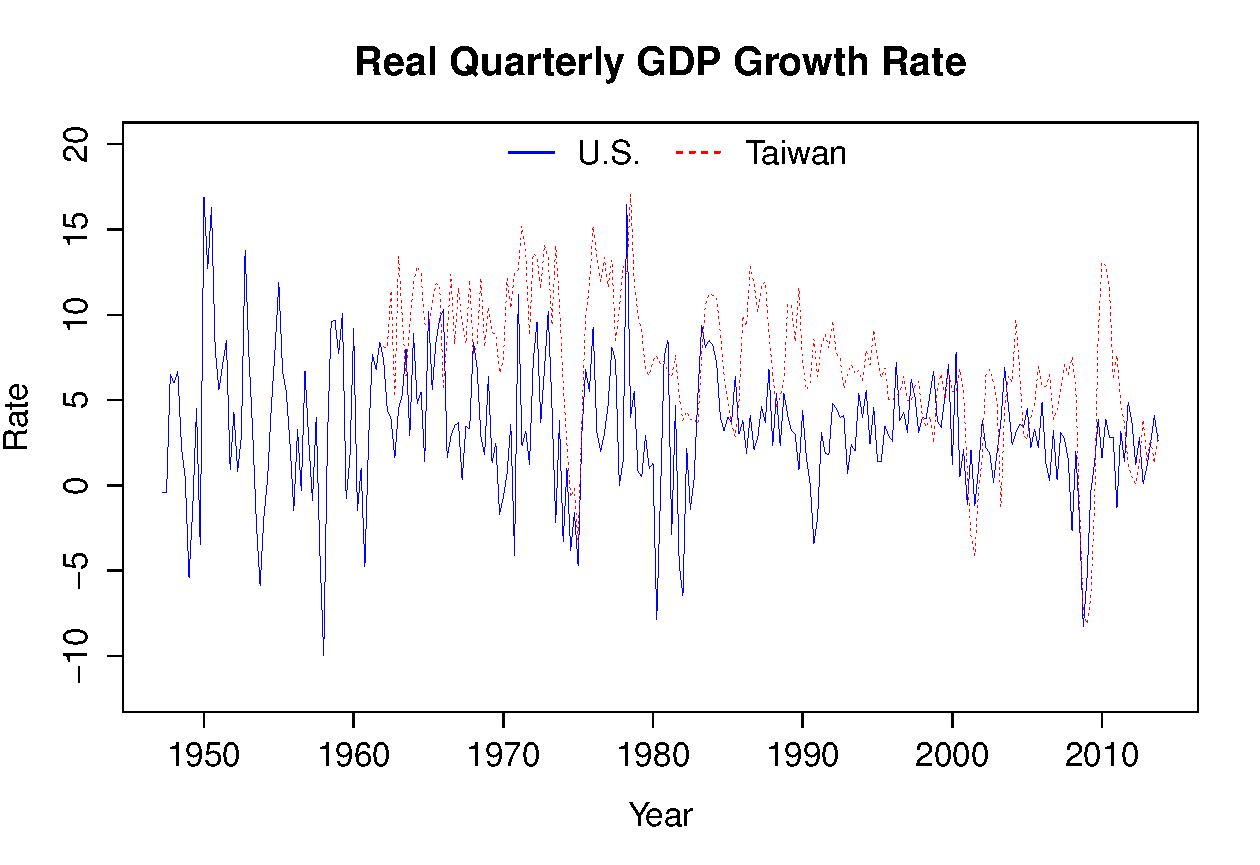
\includegraphics[scale=0.7]{gdp_ts.pdf}
	\label{fig1}
\end{figure}
\subsection{Forecast U.S. GDP Growth}
Here we apply our method to forecasting U.S. GDP growth rate\footnote{The data we use for this application are from Bruce Hansen's website:\url{http://www.ssc.wisc.edu/~bhansen/cbc/}. Hansen has several exogenous predictors included in his data in addition to the GDP growth data.} out-of-sample and compare its performance with others. We have quarterly data from 1960:1 to 2012:1, 209 total observations. The variable we are interested in forecasting is the U.S. quarterly GDP growth rate. Predictors included in some models are the quarterly change of U.S. 3-month treasury rate ($\Delta\mathrm{SR}$), the quarterly change of U.S. 10-year treasury rate ($\Delta\mathrm{LR}$) and the quarterly change of default premium ($\Delta\mathrm{DP}$)\footnote{In the database, these predictors are given in levels, but we have converted them to rates of change, so the actual sample size in all models except for the AR(1) is 207. The default premium is calculated by the difference between the AAA bond rate and BAA bond rate.}.

We consider five models, from small to large they are:
\begin{subequations}
\begin{align}
\Delta\mathrm{GDP}_{t} & = \beta_{0} + \beta_{1}\Delta\mathrm{GDP}_{t-1} + \epsilon_{t} \label{md:1}\\
\Delta\mathrm{GDP}_{t} & = \beta_{0} + \beta_{1}\Delta\mathrm{GDP}_{t-1} + \beta_{2}\Delta\mathrm{GDP}_{t-2} + \epsilon_{t}\label{md:2} \\
\Delta\mathrm{GDP}_{t} & = \beta_{0} + \beta_{1}\Delta\mathrm{GDP}_{t-1} + \beta_{2}\Delta\mathrm{SR}_{t-1} + \epsilon_{t}\label{md:3} \\
\Delta\mathrm{GDP}_{t} & = \beta_{0} + \beta_{1}\Delta\mathrm{GDP}_{t-1} + \beta_{2}\Delta\mathrm{SR}_{t-1} + \beta_{3}\Delta\mathrm{LR}_{t-1} + \epsilon_{t}\label{md:4} \\
\Delta\mathrm{GDP}_{t} & = \beta_{0} + \beta_{1}\Delta\mathrm{GDP}_{t-1} + \beta_{2}\Delta\mathrm{SR}_{t-1} + \beta_{3}\Delta\mathrm{LR}_{t-1} + \beta_{4}\Delta\mathrm{DP}_{t-1} + \epsilon_{t}\label{md:5}
\end{align}
\end{subequations}
Since in reality we do not know the ``true'' econometric model specification, we consider the above five candidate models. For each model, we examine the performance of various model averaging methods. Consistent with what is done in the previous simulation section, for each model we use the recursive window to forecast out-of-sample. To better examine the OOS performance, in each case we generate a sequence of RMSFE by varying the evaluation sample size, from 20 to 50, with increments of 5. Forecast results from all five models are presented in table~\ref{ntb:3}. For simplicity and ease of comparison, following our Monte Carlo simulation we pick the equal weight method as the benchmark and normalize all OOS forecasting performance around $1$. If the value of relative RMSFE is below $1$, then the OOS forecasts perform better than that of the equal weight method.

We can see that in all five models approximating the DGP, CV forecasts better than SIC, Cp and equal weight under recursive window across all evaluation sample sizes. Additionally, CV is the only method which beats equal weight. The forecast gains of CV relative to equal weight range from about $1\%$ to $6\%$ across evaluation sample sizes and models. CV solves the forecast combination puzzle in this application.

\begin{table}
    \caption{U.S. Quarterly GDP Growth Rate Forecast Comparison} \label{ntb:3}
    \centering
    \begin{adjustbox}{width=\textwidth,totalheight=\textheight,keepaspectratio}
    \begin{threeparttable}
    \begin{tabular}{lccccccccccccccc}
    \toprule
     & \multicolumn{3}{c}{Model a} & \multicolumn{3}{c}{Model b} & \multicolumn{3}{c}{Model c} & \multicolumn{3}{c}{Model d} & \multicolumn{3}{c}{Model e}\\%[0.3em]
    \cmidrule(r){2-4}
    \cmidrule(r){5-7}
    \cmidrule(r){8-10}
    \cmidrule(r){11-13}
    \cmidrule(r){14-16}\\
           & Cp    & CV    & SIC  & Cp    & CV    & SIC & Cp    & CV    & SIC & Cp    & CV    & SIC & Cp    & CV    & SIC \\
    P = 20 & 1.044 & 0.967 & 0.999& 1.031 & 0.983 &0.999& 1.017 & 0.987 &0.999& 1.038 & 0.970 &0.998& 1.043 & 0.960 &0.997 \\
    P = 25 & 1.038 & 0.968 & 0.999& 1.021 & 0.984 &0.999& 1.036 & 0.976 &0.999& 1.038 & 0.969 &0.998& 1.017 & 0.967 &0.998 \\
    P = 30 & 1.022 & 0.977 & 0.999& 1.022 & 0.983 &0.999& 1.007 & 0.996 &1.000& 1.013 & 0.991 &0.998& 1.032 & 0.975 &0.998 \\
    P = 35 & 1.020 & 0.980 & 1.000& 1.036 & 0.996 &0.999& 1.022 & 0.983 &0.999& 1.024 & 0.983 &0.999& 1.034 & 0.973 &0.998 \\
    P = 40 & 1.022 & 0.979 & 0.999& 1.012 & 0.987 &1.000& 1.024 & 0.982 &0.999& 1.025 & 0.982 &0.999& 1.033 & 0.974 &0.998 \\
    P = 45 & 1.024 & 0.978 & 1.000& 1.014 & 0.986 &1.000& 1.025 & 0.982 &0.999& 1.026 & 0.981 &0.999& 1.037 & 0.974 &0.998 \\
    P = 50 & 1.021 & 0.987 & 1.000& 1.011 & 0.989 &1.000& 1.027 & 0.984 &0.999& 1.023 & 0.987 &0.999& 1.022 & 0.988 &0.999 \\
    \bottomrule
    \end{tabular}
    \begin{tablenotes}[para, flushleft] \footnotesize
    Notes: Quarterly data from 1960:1 to 2012:1. $\mathrm{P}$ is the evaluation sample size. Equal weight is chosen as the benchmark and the numbers in the table represent the RMSFE ratio between each individual method and equal weight. Smaller number indicates better forecasting performance. Cp: Mallows' weights. CV: cross-validation weights. SIC: Schwarz-Bayesian weights.
    \newline Model a: AR(1)
    \newline Model b: AR(2)
    \newline Model c: AR(1) + SR
    \newline Model d: AR(1) + SR + LR
    \newline Model e: AR(1) + SR + LR + DP
    \end{tablenotes}
    \end{threeparttable}
    \end{adjustbox}
\end{table}
%Since in this section we are only interested in comparing our methods with others and in trying to somehow solve the forecast combination puzzle, we do not select one best model approximating %the DGP among those five candidates listed above. In practice, researcher may select a best
\subsection{Forecast Taiwan GDP Growth}
Here we apply our method to forecasting Taiwan GDP growth rate out-of-sample and compare its performance with others. We have quarterly data from 1962:1 to 2013:4, 208 total observations. The variable we are interested in forecasting is the Taiwan quarterly GDP growth rate. Since we do not have any exogenous predictors available, we only consider two AR forecasting models, namely, the AR(1) model and the AR(2) model. We continue the general setting outlined in the previous application. For each model, we generate a sequence of RMSFE by varying the evaluation sample size, from 20 to 50, with increments of 5. Forecast results from all five models are shown in table~\ref{ntb:5}. For simplicity and ease of comparison, following our Monte Carlo simulation we pick the equal weight method as the benchmark and normalize all OOS forecasting performance around $1$. If the value of relative RMSFE is below $1$, then the OOS forecasts perform better than that of the equal weight method.

From table~\ref{ntb:5}, we can see that now the Mallows' weights do better than the equal weight in both models and across all evaluation sample sizes. For the AR(1) model, all three methods perform roughly the same but CV has the smallest RMSFE ratio across all evaluation sample sizes. For the AR(2) model, CV performs significantly better than the other two methods.
\begin{table}
    \caption{Taiwan Quarterly GDP Growth Rate Forecast Comparison} \label{ntb:5}
    \centering
    \begin{adjustbox}{keepaspectratio}
    \begin{threeparttable}
    \begin{tabular}{lcccccc}
    \toprule
     & \multicolumn{3}{c}{Model AR(1)} & \multicolumn{3}{c}{Model AR(2)}\\%[0.3em]
    \cmidrule(r){2-4}
    \cmidrule(r){5-7}\\
           & Cp    & CV    & SIC  & Cp    & CV    & SIC  \\
    P = 20 & 0.991 & 0.947 & 0.999& 0.968 & 0.944 &1.000\\
    P = 25 & 0.998 & 0.994 & 1.000& 0.972 & 0.942 &1.000\\
    P = 30 & 0.998 & 0.995 & 1.000& 0.973 & 0.943 &1.000\\
    P = 35 & 0.999 & 0.995 & 1.000& 0.974 & 0.945 &1.000\\
    P = 40 & 0.998 & 0.993 & 1.000& 0.976 & 0.948 &1.000\\
    P = 45 & 0.998 & 0.993 & 1.000& 0.982 & 0.961 &1.000\\
    P = 50 & 0.997 & 0.996 & 1.000& 0.984 & 0.962 &1.000\\
    \bottomrule
    \end{tabular}
    \begin{tablenotes}[para, flushleft] \footnotesize
    Notes: Quarterly data from 1962:1 to 2013:4. $\mathrm{P}$ is the evaluation sample size. Equal weight is chosen as the benchmark and the numbers in the table represent the RMSFE ratio between each individual method and equal weight. Smaller number indicates better forecasting performance. Cp: Mallows' weights. CV: cross-validation weights. SIC: Schwarz-Bayesian weights.
    \end{tablenotes}
    \end{threeparttable}
    \end{adjustbox}
\end{table} 